The previous section discussed the generation of a hard process
according to lowest-order matrix elements.  These describe the momenta of
the outgoing jets well, but to give an exclusive picture of the process,
including the internal structure of the jets and the distributions of
accompanying particles, any fixed order is not sufficient.  The effect
of all higher orders can be simulated through a parton shower algorithm,
which is typically formulated as an evolution in momentum transfer down
from the high scales associated with the hard process to the low scales,
of order 1~GeV, associated with confinement of the partons it describes
into hadrons.

In this section, we describe the physics behind parton showering.  Much
of our language will be based on the conventional approach in which a
parton shower simulates a succession of emissions from the incoming and
outgoing partons.  Towards the end of the section, however, we will
describe a slightly different formulation based on a succession of
emissions from the coloured dipoles formed by pairs of these
partons.  As we will discuss there, at the level of detail of our
presentation, the two approaches are almost equivalent and most of this
section applies equally well to dipole-based showers.

\mcsubsection{Introduction: QED bremsstrahlung in scattering processes}

We are familiar with the fact that in classical electrodynamics charges
radiate when scattered (see for example \cite{jackson1999},~chapter 15).
Calculating a scattering process in perturbative QED, one finds that the
radiation pattern of photons at the first order agrees with this
classical calculation (an important fact proved in Low's
theorem~\cite{Low:1958sn}).  One also encounters loop diagrams, which
correct the non-emission process such that the sum of emission and
non-emission probabilities is unity.  At successively higher
orders, soft photons are effectively emitted independently.
The spectrum extends down to arbitrarily low
frequencies, so that the total number of photons emitted is ill-defined,
but the number of observable
photons above a given energy is finite.  The probability of no
observable photons is also finite, and exponentially suppressed for
small energy cutoffs (known as Sudakov suppression~\cite{Sudakov:1954sw}).

One important property of this QED bremsstrahlung is the fact that
emission from different particles involved in the same scattering event
is coherent.  One manifestation of this is that when a high energy
photon produces an $e^+e^-$ pair in the field of a nucleus and, due to
the high boost factor, the pair are extremely close to each other in
direction, they do not ionize subsequent atoms they pass near because,
while they are closer together than the atomic size, the atoms only see
their total charge, which is zero, and not their individual charges.
Only once their separation has reached the atomic size do they start to
ionize.  In effect, the charged particles only behave independently with
respect to observers in a forward cone of opening angle given by their
separation and at larger angles they behave as a coherent pair.  This is
observed in bubble-chamber photographs as a single line of very weak
ionization that becomes stronger and eventually separates into two lines
and is known as the Chudakov effect~\cite{Chudakov:55ce}.  We will see
that there is a corresponding effect in QCD.

Having recalled these basic features of QED bremsstrahlung, we will
calculate the equivalent processes in QCD and see many analogous
features, as well as crucial differences arising from the non-abelian
nature of QCD and the resulting strong interactions at low energy.

\mcsubsection{Collinear final state evolution}

Although the utility of parton showers comes from the fact that they are
universal (process-independent) building blocks, we find it instructive
to motivate their main features by considering a specific process,
$e^+e^-$ annihilation to jets.  The leading-order cross section is given
by the electroweak process $e^+e^-\to q\bar{q}$ and is finite.  We
define its total cross section to be~$\sigma_{q\bar q}$.

We are more interested in the next-order process, $e^+e^-\to q\bar{q}g$,
which we hope to formulate as the production of a $q\bar{q}$ pair,
accompanied by the emission of a gluon by that pair.  Parameterizing the
three-parton phase space with $\theta$, the opening angle between the
quark and the gluon, and $z$, the energy fraction of the gluon, we
obtain
\begin{equation}
  \label{sigmaeeqqg2}
  \frac{\done\sigma_{q\bar qg}}{\done\cos\theta\,\done z} \approx
  \sigma_{q\bar q} \, C_F \, \frac{\alphaS}{2\pi} \,
  \frac2{\sin^2\theta}\,\frac{1+(1-z)^2}z\,,
\end{equation}
where $C_F=\frac{\Nc^2-1}{2\Nc}$ is a colour factor that can be thought as
the colour-charge squared of a quark.  In \EqRef{sigmaeeqqg2} we see
that the differential cross section diverges at the edges of phase
space.  To illustrate this, we have approximated the full expression
(which can be found in \cite{Ellis:1991qj} for example) by neglecting
non-divergent terms.
Recalling that the bremsstrahlung distribution was also divergent in
QED, but that this did not matter for a physical description of the
final state of observable photons, this divergence may not be a problem.
But we will certainly want to understand its physical origin since, as
we approach the divergences, the emission distribution will be large and
these will be the regions that dominate the emission pattern.

In \EqRef{sigmaeeqqg2}, we also see the structure we were hoping for: the
cross section for $q\bar{q}g$ is proportional to that for $q\bar{q}$ and
therefore we may interpret the rest of the expression as the probability
for gluon emission, differential in the kinematics of the gluon.

The integrand of \EqRef{sigmaeeqqg2} can diverge in three
ways: $\theta\to0$, corresponding to the gluon being collinear to the
quark; $\theta\to\pi$, corresponding to the gluon being back-to-back
with the quark, \ie collinear with the antiquark; and $z\to0$,
the gluon energy going to zero for any value of the opening angle.  Each
of the first two divergences can be traced to a propagator in one of the
two Feynman diagrams going on-shell.  However, it should be emphasized
that \EqRef{sigmaeeqqg2} contains the sum of the two diagrams and
properly includes their interference.  The third divergence comes from
the propagators in both diagrams going on-shell simultaneously and much
more clearly involves the interference of the two diagrams.  We return
to discuss the soft region in \SecRef{parton-showers:soft-gluons} and
for now focus on the collinear regions.

We can separate the angular distribution into two components, each of
which is divergent in only one of the two collinear regions,
\begin{equation}
  \frac2{\sin^2\theta} = \frac1{1-\cos\theta} + \frac1{1+\cos\theta}
  \approx \frac1{1-\cos\theta} + \frac1{1-\cos\bar\theta},
\end{equation}
where $\bar\theta$ is the angle between $g$ and $\bar{q}$ and the
approximation is as good as the one in \EqRef{sigmaeeqqg2}.  The
distribution can therefore be written as the sum of two separate
distributions, describing the emission of a gluon close to the
directions of the quark or the antiquark.  Since the distributions are
summed, they are effectively independent.  We emphasize again though,
that they are derived from the proper sum of amplitudes for diagrams in
which the gluon is attached to either emitter; it is just convenient to
separate them into pieces that can be treated independently.

We can therefore write the emission distribution as
\begin{equation}
  \label{firstcollinear}
  \done\sigma_{q\bar qg} \approx \sigma_{q\bar q} \sum_{\mathrm{partons}}
  C_F \, \frac{\alphaS}{2\pi} \, \frac{\done\theta^2}{\theta^2}
  \, \done z\frac{1+(1-z)^2}z,
\end{equation}
where now $\theta$ is the opening angle between the gluon and the parton
that emitted it.  This is starting to look like something that can be
implemented and iterated in a Monte Carlo algorithm, with an independent
emission distribution for each parton.  Before generalizing it, we point
out one mathematically-trivial property of this equation, which will
turn out to be important for the physical properties of our parton
shower algorithm.  In writing down \EqRef{firstcollinear}, we have
focused on the small-$\theta$ region, which gives the collinear
divergence.  However, we would have obtained a mathematically-identical
expression if we had chosen to parameterize the phase space in terms of
any other variable proportional to $\theta^2$, for example the
virtuality of the off-shell quark propagator,
$q^2=z(1-z)\,\theta^2\,E^2$, where $E$
is its energy, or the gluon's transverse momentum with respect to the
parent quark's direction,
$\kt^2=z^2(1-z)^2\,\theta^2\,E^2$, since
\begin{equation}
  \label{eq:evolchoices}
  \frac{\done\theta^2}{\theta^2} = \frac{\done q^2}{q^2} =
  \frac{\done\kt^2}{\kt^2}.
\end{equation}
Any of these forms would give identical results in the collinear limit,
but different extrapolations away from it, \ie different finite terms
accompanying the divergence.

While it is not obvious from our derivation, the structure of
\EqRef{firstcollinear} is completely general.  For any hard process that
produces partons of any flavour $i$, the cross section for a hard
configuration that has cross section $\sigma_0$ to be accompanied by a
parton $j$ with momentum fraction $z$ is given by
\begin{equation}
  \label{collinear}
  \done\sigma \approx \sigma_0 \sum_{\mathrm{partons},i}
  \frac{\alphaS}{2\pi} \, \frac{\done\theta^2}{\theta^2}
  \, \done z\,P_{ji}(z,\phi) \done\phi,
\end{equation}
with $P_{ji}(z,\phi)$ a set of universal, but flavour-dependent (and,
through $\phi$, the azimuth of $j$ around the axis
defined by $i$, spin-dependent) functions.  The spin-dependence can be
found in, for example, Ref.~\cite{Ellis:1991qj}~-- we give the
spin-averaged functions:
\begin{equation}
  \label{DGLAP}
  \begin{array}{rcl@{\hspace*{2.5em}}rcl}
    P_{qq}(z) &=& C_F\,\frac{1+z^2}{1-z}, &
    P_{gq}(z) &=& C_F\,\frac{1+(1-z)^2}z, \\
    P_{gg}(z) &=& C_A\,\frac{z^4+1+(1-z)^4}{z(1-z)}, &
    P_{qg}(z) &=& T_R(z^2+(1-z)^2),
  \end{array}
\end{equation}
where $C_F$ was already defined above, $C_A=\Nc$ is a colour factor that
can be thought as the colour-charge squared of a gluon, and $T_R$
is a colour factor that is fixed only by convention, $T_R=\frac12$ (a
different value of $T_R$ would be compensated by a different definition
of $\alphaS$).  $P_{qq}$, $P_{gq}$, $P_{gg}$ and $P_{qg}$ correspond to the
splittings $q\to qg$, $q\to gq$, $g\to gg$ and $g\to q\bar{q}$
respectively\footnote{A fifth splitting function $P_{\bar{q}g}$
  corresponding to $g\to\bar{q}q$  is equal to $P_{qg}$ by symmetry.}.
In the collinear limit, in which these results are valid, they are
independent of the precise definition of $z$~-- it could be the energy
fraction, light-cone momentum fraction, or anything similar, of parton
$j$ with respect to parton~$i$.
We now have the basic building block to write an iterative algorithm:
since \EqRef{collinear} is a completely general expression for any hard
process to be accompanied by a collinear splitting, we can iterate it,
using it on the hard process to generate one collinear splitting and
then treating the final state of that splitting as a new hard process,
generating an even more collinear splitting from it, and~so~on.

However, we are not quite ready to do so yet, because we have not yet
learnt how to deal with the divergence.  We have seen where it comes
from and that it is universal, but not how to tame it to produce a
well-defined probability distribution.  This comes when we ask what we
mean by a final-state parton.  The point is that any physical
measurement cannot distinguish an exactly collinear pair of partons from
a single parton with the same total momentum and other quantum numbers.
The infinitely high probability is associated with a transition that has
no physical effect.  As in our discussion of QED, to produce
physically-meaningful distributions, we should introduce a resolution
criterion, saying that we will only generate the distributions of
resolvable partons.  A particular convenient choice, although by no
means the only one possible, is the transverse momentum: to say that two
partons are resolvable if their relative transverse momentum is above
some cutoff~$Q_0$.  This cuts off both the soft and collinear
divergences, and gives a total resolvable-emission probability that is
finite.  To calculate the non-resolvable-emission probability, one must
integrate the emission distribution below the cutoff and add it to the
loop-correction to the hard process.  The result is finite, but there is
an easier way to obtain it: unitarity tells us that the total
probability of \emph{something\/} happening, either emission or
non-emission, is unity, and therefore, knowing the emission probability,
we can calculate the non-emission probability as one minus it.  (This
unitarity argument is exact in the case of soft or collinear emission,
but in general hard non-collinear loops contribute a finite correction,
which can be absorbed into the normalization of the total cross section,
restoring unitarity.)
It is sometimes said that parton shower algorithms do not include loop
corrections, but if this were so the non-emission probability would be
ill-defined.  It is better to say that they construct the loop
corrections by unitarity arguments from the tree corrections.

We are almost ready to construct the probability distribution for one
emission from a hard process, the basic building block that we will
iterate to produce a parton shower.  To do this, we have to realize that
the distribution we have been calculating so far is the inclusive
emission distribution of all gluon emissions: their total energy is the
total energy carried away by all gluons emitted, given by the classical
result.  To calculate instead the distributions of exclusive multi-gluon
events, it is convenient to separate out the distributions of individual
gluons, for example by introducing an ordering variable.  Let us take as
an illustrative
example, the virtuality of the internal line, $q^2$.  The distribution
we have been calculating is the total probability for all branchings of
a parton of type $i$ between $q^2$ and $q^2+\done q^2$,
\begin{equation}
  \done\mathcal{P}_i=\frac{\alphaS}{2\pi}\,\frac{\done q^2}{q^2}
  \int_{Q_0^2/q^2}^{1-Q_0^2/q^2}\done z\,P_{ji}(z),
\end{equation}
where the limits on $z$ come from the requirement that the partons be
resolvable, and their precise form depends on the definition of the
resolution criterion and of~$z$.
In order to construct the probability distribution of the
first branching, \ie the one that yields the largest contribution to the
virtuality of the internal line, we need to calculate the probability
that there are no branchings giving virtualities greater than a given
$q^2$ value, given that it has a maximum possible virtuality of $Q^2$.
We define this function to be $\Delta_i(Q^2,q^2)$.  It is given by a
differential equation,
\begin{equation}
  \label{q^2distribution}
  \frac{\done\Delta_i(Q^2,q^2)}{\done q^2} = \Delta_i(Q^2,q^2)\,
  \frac{\done\mathcal{P}_i}{\done q^2},
\end{equation}
corresponding to the fact that, when changing $q^2$ by a small amount,
the probability $\Delta_i$ can only change by the branching probability
$\done\mathcal{P}_i$ if there are no branchings above $q^2$, which
has probability $\Delta_i$.  It is easy to check that this equation has
the solution
\begin{equation}
  \label{Sudakov}
  \Delta_i(Q^2,q^2) = \exp\left\{-\int_{q^2}^{Q^2}\frac{\done k^2}{k^2}\,
  \frac{\alphaS}{2\pi} \int_{Q_0^2/k^2}^{1-Q_0^2/k^2}\done z\,P_{ji}(z)
  \right\}\,.
\end{equation}
This formula has a close analogy with the well-known radioactivity decay
formula: if the rate of decay of nuclei is $\lambda$ per unit time, then
the probability that a given nucleus has not decayed by time $T$ is
given by $\exp\left\{-\int_0^T\done t\,\lambda\right\}$.  Or, in words,
the probability of non-branching over some region is given by $e$ to
the minus the total inclusive branching probability over that region.

A particular case of this non-branching probability is
$\Delta_i(Q^2,Q_0^2)$, the total probability to produce \emph{no\/}
resolvable branchings.  This is the Sudakov form factor we encountered in
our discussion of QED, given by
\begin{eqnarray}
  \label{exponentiation}
  \Delta_i(Q^2,Q_0^2) &=& \exp\Biggl\{-\int_{Q_0^2}^{Q^2}\frac{\done k^2}{k^2}\,
  \frac{\alphaS}{2\pi} \int_{Q_0^2/k^2}^{1-Q_0^2/k^2}\done z\,P_{ji}(z)
  \Biggr\} \\
  &\sim& \exp\Biggl\{-C_F\,\frac{\alphaS}{2\pi}\log^2\frac{Q^2}{Q_0^2}
  \Biggr\}\,,
\end{eqnarray}
for a quark, a probability that falls faster than any inverse power of
$Q^2$.

Finally, we have the building block we need to iteratively attach
additional partons to a hard process one at a time.  Since $\Delta_i$
describes the probability to have no branching above $q^2$, its
derivative, the right-hand-side of \EqRef{q^2distribution}, is the
probability distribution for the first branching.  Having produced such
a branching, the same procedure has to be applied to each of the child
partons, with their $q^2$ values required to be smaller than the one we
generated for this splitting, to prevent double-counting.  Evolution
continues until no more resolvable branchings are produced above $Q_0^2$.
The only missing ingredient now is the starting condition: the value of
$Q^2$ for the parton line that initiated the shower, which we return to
in \SecRef{parton-shower:initial-conditions}.

The Monte Carlo implementation of \EqRef{q^2distribution} is remarkably
straightforward in principle: a random number $\rho$ is chosen between
0~and~1 and the equation $\Delta_i(Q^2,q^2)=\rho$ is solved for $q^2$.  If
the solution is above $Q_0^2$, a resolvable branching is generated at scale
$q^2$ and otherwise there is no resolvable branching and evolution
terminates.  For a resolvable branching a $z$ value is chosen according to
$P_{ji}(z)$.  Such a shower algorithm implements numerically the all-order
summation inherent in the exponentiation of \EqRef{exponentiation}.
Since this correctly sums the terms with the greatest number of logs of
$Q_0^2$ at each order of $\alphaS$ it is called a leading collinear
logarithmic parton shower algorithm.

However, there are considerable ambiguities in constructing such an
algorithm.  We already mentioned that an identical form would be given
by any other choice of evolution scale proportional to $\theta^2$, we
simply chose $q^2$ as an illustrative example.  We also defined $z$ to
be the energy fraction of the emitted parton, but in fact in the exactly
collinear limit in which \EqRef{collinear} is valid, choosing the
longitudinal momentum fraction, the light-cone momentum fraction, or
anything else similar, would give identical results, but different
extrapolations away from that limit.  Finally, since the hard process
matrix element deals with on-shell partons, and the parton shower
process has generated a virtuality for the parton line, energy-momentum
must be shuffled between partons in some way to be conserved, but the
collinear approximation does not specify how this should be done. All
of these are formally allowable choices, with the same leading
collinear logarithmic accuracy, but they differ in the amount of
subleading terms they introduce.  In the case of the evolution scale,
we will see in \SecRef{parton-showers:soft-gluons} that a study of the
soft limit of QCD matrix elements gives us an indication of the best
choice.

Before turning to the soft limit, we discuss one important source of
higher-order corrections, namely running coupling effects.  A certain
tower of higher-order diagrams, including those with loops inserted into
an emitted gluon, can be summed to all orders and absorbed by the
simple replacement of $\alphaS$ by $\alphaS(\kt)$, the running
coupling evaluated at the scale of the transverse momentum of the
emitted gluon~\cite{Amati:1980ch}.  This can be easily absorbed into the
algorithm above,
but has a couple of important consequences.  Firstly, parton
multiplication becomes much faster: as $q^2$ decreases, $\alphaS$
becomes larger and it becomes easier to emit further gluons until at
small enough scales the emission probability becomes of order~1 and
phase space fills with soft gluons.  Secondly, since one has to avoid
the region for which $\alphaS$ becomes of order~1, $Q_0$ has to be
considerably above $\LambdaQCD$, and actually becomes a physical
parameter affecting observable distributions at the end of the parton
shower, rather than a purely technical cutoff parameter that can be
taken as small as one likes, as it is without running coupling effects.
These facts mean that in the parlance used in analytical resummation,
the parton shower is not a purely perturbative description but induces
power corrections $\sim(Q_0/Q)^p$, contributing to the non-perturbative
structure of the final state. Here $p\ge1$ is a constant that may depend on
the parton shower algorithm used and the observable calculated; usually
$p=1$.

The ingredients described in this section are sufficient to construct a
final-state collinear parton shower algorithm.  However, recall that in
\mbox{$e^+e^-\to q\bar{q}g$} (\EqRef{sigmaeeqqg2}) we found that the
matrix elements were enhanced in both the
collinear and soft limits.  In order to give a complete description of
all dominant regions of the emission distribution, we should consider
soft emission in as much detail.

\mcsubsection{Soft gluon emission}
\label{parton-showers:soft-gluons}
In studying the matrix elements for $e^+e^-$ annihilation to
$q\bar{q}g$, we discovered that they were divergent as the gluon energy
goes to zero, in any direction of emission, as well as in the collinear
limit.  One may also show that this soft divergence is a general feature
of QCD amplitudes and also that it can be written in a universal factorized
form.  However, the big difference relative to the collinear case is
that the factorization is valid at the amplitude level: the
amplitude is given by the product of the amplitude to produce the system
of hard partons, times a universal factor describing the emission of the
additional gluon.  The cross section is calculated by summing all
Feynman diagrams and squaring and in practice many diagrams contribute
at a similar level, so that interference terms between diagrams are
unavoidable.  This tells us that soft gluons should be considered to be
emitted by the scattering process as a whole, rather than any given
parton, and appears to spoil the picture of independent evolution of
each parton.

Consider, as a concrete example, the configuration shown in
\FigRef{fig:softgluoncoherence}.  A quark has been produced in a hard
process and has gone on to emit a reasonably hard, but reasonably
collinear, gluon, and we wish to calculate the probability that this
event is accompanied by a soft wide-angle gluon.  The soft factorization
theorem tells us that the amplitude for this process should be
calculated as the sum of amplitudes for the gluon to be attached to each
of the external partons, as indicated by the two placements of the gluon
on the left-hand-side of the figure.  The two resulting amplitudes are
of exactly the same order and have a non-trivial phase structure, so
that interference between them seems absolutely crucial.  It appears
impossible to reconcile this with the picture of independent collinear
evolution discussed in the previous section.
\begin{figure}
  \centerline{%
    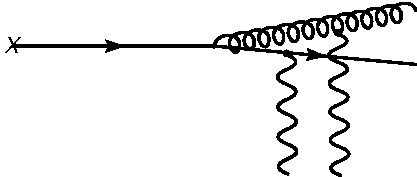
\includegraphics[width=5cm]{parton-showers/coherence1.pdf}
    \hfill
    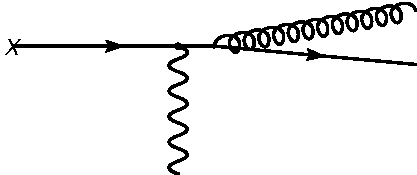
\includegraphics[width=5cm]{parton-showers/coherence2.pdf}}
  \caption{Illustration of QCD coherence. The emission of a soft
    wide-angle gluon receives contributions from Feynman diagrams in
    which it is attached to any of the external partons (left). The
    coherent sum of these diagrams is equal to the emission from a
    single parton with the total momentum and colour of the
    partons. That is, as if it were emitted before the smaller-angle
    harder gluon (right).}
  \label{fig:softgluoncoherence}
\end{figure}

However, the coherence that we discussed in the context of QED
brems\-strahlung comes into play here and shows us that we \emph{can\/}
formulate soft emission within a parton shower approach.  Explicitly
calculating the amplitudes described above, one can show that in the
region shown in the figure, in which the softer gluon is at a larger
angle than the harder one, the interference is largely destructive,
reducing the emission distribution from the level it would be if
the two partons emitted independently to a term proportional to $C_F$.
Specifically, the result is identical to the one that would be obtained
from a configuration in which the collinear quark/gluon pair is replaced
by a single \emph{on-shell\/} quark with the same total longitudinal
momentum.  That is, we can think of the wide-angle emission as being
\emph{as if\/} it occurred before the more collinear one, summarized
pictorially in the right-hand side of \FigRef{fig:softgluoncoherence}.
However, it should be emphasized that this picture is the summary of the
proper interference between quantum mechanical amplitudes and does not
represent a Feynman diagram in which the gluon is emitted by the
internal line.  This should remind us of the Chudakov effect in QED:
there, wide angle emission from the $e^+e^-$ pair was absent, because
their total charge is zero.  Here, since the gluon is itself coloured,
the emission pattern is more complicated, but the result is the same:
the soft wide angle gluon sees the \emph{total\/} colour charge of the
system of partons to which it is attached.

On the other hand, calculating the case in which the angle between the
soft gluon and one of the other partons is much smaller than that
between them, one finds that the two contributions have very different
sizes and the cross section can be described as the sum of independent
emissions from the two partons.  These considerations can easily be
generalized to systems of more than two emitting partons.  They can be
summarized in a remarkably simple result: soft gluon effects can be
correctly taken into account by a collinear parton shower algorithm,
provided that, out of the choice of all possible evolution scales, one
uses the opening angle.  This is the central result that leads to
angular-ordered, or coherence-improved, parton showers, such as is
implemented in \herwig.  As a result, the first emission in the shower
is often not the hardest and it often happens that several soft
wide-angle gluons are emitted before the hardest gluon in the shower, a
fact that will lead to some complications when we try to match with
matrix element calculations in \SecRef{sec:me-nlo-matching}.

In \SecRef{sec:dipoles}, an alternative implementation of colour
coherence is discussed, based on colour dipoles between pairs of
emitters.  It is explained there that, at the level of detail discussed
here, the \kt-ordered dipole showers and angular-ordered parton showers
are effectively equivalent.

\mcsubsection{Initial state evolution \label{sec:isr}}
So far we have discussed the evolution of the partons produced in a hard
process.  According to the analogy with QED, we equally expect partons
to radiate on their way in to a scattering or annihilation process,
giving rise to an initial-state parton shower.  In principle, the
generation of initial-state showers can be set up in an extremely
similar way to the final-state showers already discussed, with an
incoming parton evolving through a series of $1\to2$ splittings to a
shower of partons, one of which is ultimately involved in the hard
process, with the rest being emitted as accompanying radiation.
An added complication in the initial-state case is that whole showers,
and branches off the sides of showers, can develop that do not
ultimately participate in any hard scatter.  These should be collapsed
back into the proton remnant in the same way that fluctuations that
develop in a freely-moving proton that does not have any interaction
collapse back into it.

In practice, simulating initial-state showers in this way is extremely
inefficient, because the majority
of partons have low energy and virtuality and if the showers were
produced with the same frequency as in nature, it would be extremely
rare to produce exactly the right kinematics to produce a hard process
of interest, such as Higgs production.  Moreover, as we shall discuss in
\SecRef{parton-shower:initial-conditions}, the properties of the parton
showers, both initial- and final-state, are correlated with the hard
process, and it would be difficult to build this in to such an
initial-state shower.  Instead,
event generators actually start by selecting the hard process and then
using the parton shower evolution to dress it with additional radiation.
That is, our basic building block is a \emph{backwards\/} step: one
generates the probability distribution for a parton with given momentum
fraction and value of evolution scale to have come from one at a higher
momentum fraction and lower scale.  This is iterated
until the evolution scale reaches the infrared cutoff, whereupon a
non-perturbative model of the remnant left behind by the extraction of a
parton from the incoming hadron is invoked.

The evolution of the PDFs with momentum
scale is given by the DGLAP
equations~\cite{Gribov:1972ri,Dokshitzer:1977sg,Altarelli:1977zs}.  They
can be viewed as
describing the flow of information about the PDFs to a given point in the
$(x,Q^2)$ plane from a boundary condition, usually a fixed line at some
input scale $Q^2=Q_0^2$, requiring information about all higher values
of $x$.  As pointed out in \cite{Sjostrand:1985xi} and further developed in
\cite{Marchesini:1987cf}, one can use the solution to the DGLAP
equations to guide the
backward evolution just described.  That is, for a parton of a given
flavour at a given $x$ and $q^2$ value, we can calculate the conditional
distribution that it came from a parton of the same or another flavour
at a higher $x$ and lower $q^2$ value.  Moreover, at leading order, this
distribution is positive definite and we can formulate it as a
probabilistic Markov chain.  The final result, which we do not derive
here (see the original references, \cite{Sjostrand:1985xi,Marchesini:1987cf}), is that the Sudakov form
factor, $\Delta_i(Q^2,q^2)$
(\EqRef{Sudakov}), which gives the probability that a final-state parton
does not produce any radiation at scales between $q^2$ and $Q^2$, is
replaced in the initial-state case\footnote{Note the interchange of the
  $ij$ indices on $P_{ij}$ relative to the final-state case, which comes
  about because this is a backward evolution.} by a non-emission
probability $\Delta_i(Q^2,q^2;x)$,
\begin{equation}
  \label{ISRsudakov}
  \!
  \Delta_i(Q^2,q^2;x) = \exp\left\{-\int_{q^2}^{Q^2}\frac{\done k^2}{k^2}\,
  \frac{\alphaS}{2\pi} \int_{Q_0^2/k^2}^{1-Q_0^2/k^2}\done z\,P_{ij}(z)
  \, \frac{x/z\,f_j(x/z,k^2)}{x\,f_i(x,k^2)}
  \right\}.
  \!\!
\end{equation}
The inclusive emission probability, which gets exponentiated to give the
non-emission probability, contains an extra factor of the ratio of
parton distribution functions at the `new', higher, value of $x$ that
the parton may evolve back to and its `current' value.
Thus, if our parton is in a region
in which the PDF decreases rapidly with increasing $x$, its non-emission
probability will be close to one, \ie its emission probability will be
small, and it is more likely that the parton came straight out of the
hadron at the infrared cutoff scale, rather than having been produced by
evolution of a higher-$x$ parton.  In the same way, if an emission is
generated, its $z$ value is not generated according to $P_{ij}(z)$, but
rather includes an extra factor of $x/z\,f_j(x/z,k^2)$.  In this way, one
can show that the algorithm is guaranteed to follow the same evolution
as the input parton distributions, provided the limit $Q_0\to0$ is
taken.  In reality, it is modified somewhat by infrared (\ie finite
$Q_0$) effects.  In addition, the emitted partons go on to produce
final-state parton showers of their own.

The arguments concerning the coherence of radiation from different
emitters and the scale of the running coupling apply equally well to
initial-state showers.  Indeed, one can show that along the
initial-state line, the opening angle of each emission relative to the
fixed direction of the incoming hadron is the correct ordering
variable \cite{Marchesini:1987cf} in a parton shower algorithm
and that the showers produced by the emitted
partons should have opening angles limited also by this angle.  Again
the appropriate scale for the running coupling is the transverse
momentum of emitted gluons.  Ref.~\cite{Catani:1990rr} showed that,
if these conditions are met, then the shower algorithm, even with LO
splitting functions, is correct to NLO accuracy in the limited phase
space region $x\to1$.
%% This accuracy allows one to understand the effective
%% scheme in which the parton shower is defined, relate it to the
%% $\overline{\mathrm{MS}}$ scheme and, in principle, use it to extract,
%% from measured scaling violations at large $x$, a value of
%% $\alphaS^{\overline{\mathrm{MS}}}(M_Z)$.  This relation is exploited in
%% \Herwigpp\ to make $\alphaS^{\overline{\mathrm{MS}}}(M_Z)$ the input
%% parameter specified by the user, but the fact that the relation is only
%% valid in a limited region of phase space makes it questionable how
%% useful in practice this relation is.  The value is still therefore
%% considered a freely adjustable parameter, not necessarily fixed to the
%% world average.

In the discussion of final-state parton showers, we emphasized that they
were derived from the full amplitudes of the theory, including
interference between different amplitudes, and describing a particular
gluon emission as being from a particular parton is a convenient
language to use, but is not truly what happens at the fundamental
level.  Since we properly include colour coherence effects, we do
account for interference between amplitudes.  The same is true for the
separation into final-state and initial-state emission: the separation
is arbitrary and only the sum of the two is physically meaningful and
reproduces the underlying quantum mechanical amplitude.  In the dipole
approach to parton showering, gluons are emitted by the colour dipole
that stretches between a colour--anticolour pair.  This picture works
also for scattered partons, where an incoming colour line behaves
effectively like an outgoing anticolour line and a scattered quark in
DIS, for example, radiates coherently with a radiation pattern that
peaks in the incoming and outgoing directions, without the need for an
explicit separation into initial- and final-state, as we shall discuss a
little more in \SecRef{sec:dipoles}.

Although not the main focus of this review, we note that for scattering
processes involving partons with very small momentum fractions (\ie at
given hard process kinematics, for very high energy incoming hadrons)
logarithms of the momentum fraction at each splitting can be large and a
different resummation is needed
(BFKL~\cite{Balitsky:1978ic,Kuraev:1977fs} or CCFM~\cite{Catani:1989sg}).
Such a resummation
can also be formulated in a probabilistic way, either as a dipole
cascade (see \SecRef{sec:ariadne}) or as a parton shower, as in the
SmallX~\cite{Marchesini:1992jw} and Cascade~\cite{Jung:2000hk} programs.
While quantifying how small a momentum fraction is needed before
including these effects becomes essential has proved elusive, it seems
very likely that a variety of hard processes at the LHC with momentum
fractions below $10^{-4\mbox{\scriptsize~or~}5}$ will be significantly
affected by them.

\mcsubsection{Connecting parton showers to the hard process}
\label{parton-shower:initial-conditions}
We have discussed the evolution of partons on their way in and out of a
scattering process, but not the starting conditions for the showers,
\ie the maximum values of $Q^2$.  Here again coherence plays a crucial
role.  In this section we discuss the simplest case of $2\to2$
scattering, but the general case is intimately linked with the question
of matrix element matching, which we discuss in detail in
\SecRef{sec:me-nlo-matching}.

A first consideration involves avoidance of double counting.  A QCD $2\to2$
scattering accompanied by an emission from one of the external legs that
is much harder than the hard scale gives the hard process a strong
recoil that boosts one or both of its outgoing partons to a significantly
higher transverse momentum.  The outcome is a configuration that is
indistinguishable from one that arises from a harder hard process
accompanied by a softer emission from one its external legs.  The fact
that one configuration can arise in two ways is a double counting and
should be resolved by only allowing one of them.  Since the parton
shower is built on the soft and collinear approximations, the
distribution of soft emission in hard scatters is more accurate than
that of hard emission in soft scatters and it is the former that should
be used.  This can be enforced by setting the upper limit of the parton
shower evolution to the scale of the hard scattering.  In the case of
processes for which the lowest order is purely electroweak, for example
gauge boson production, there is no analogous process with which hard
emission would be double-counted, but nevertheless event generators
typically also in this case limit emission to be below the hard scale,
where the parton shower approximations are most reliable, and instead
populate the region of phase space corresponding to harder emission
using matrix element corrections, as discussed
in \SecRef{sec:me-nlo-matching}.

The second consideration arises due to colour coherence.  In the limit
of a large number of colours, $\Nc\to\infty$, the colour structure of a
gluon can be considered to be a fundamental colour--anticolour pair, as
discussed in \SecRef{sec:large-nc-limit}.
In a scattering process such as $q\bar{q}\to q'\bar{q}'$, illustrated in
\FigRef{fig:hardscattercoherence}, although the flavour of the quark and
antiquark is annihilated, their colour lines flow onto the $s$-channel
gluon and hence onto the outgoing (anti)quarks, as illustrated in
\FigRef[b]{fig:hardscattercoherence}.
\begin{figure}[t]
  \centerline{\raisebox{2cm}{(a)}\!\!%
    \raisebox{0pt}{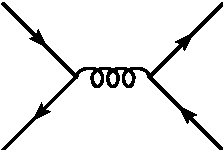
\includegraphics[width=4cm]{parton-showers/coherence3.pdf}}
    \hfill\raisebox{2cm}{(b)}\!\!
    \raisebox{-5pt}{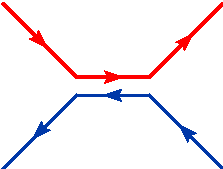
\includegraphics[width=4cm]{parton-showers/coherence4.pdf}}
    \hfill\raisebox{2cm}{(c)}\!\!
    \raisebox{30pt}{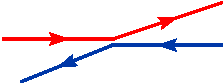
\includegraphics[width=4cm]{parton-showers/coherence5.pdf}}}
  \caption{Illustration of colour coherence effect in hard scattering
    processes. In the quark--antiquark annihilation and production
    process (a), the quark's flavour is annihilated, but its colour
    flows onto the outgoing quark (b), such that in the
    centre-of-mass system, the colours are only scattered through small
    angles (c).}
  \label{fig:hardscattercoherence}
\end{figure}
\begin{figure}[t]
  \centerline{\raisebox{2cm}{(a)}\!\!%
    \raisebox{0pt}{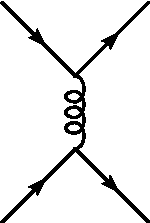
\includegraphics[width=2.7cm]{parton-showers/coherence6.pdf}}
    \hfill\raisebox{2cm}{(b)}\!\!
    \raisebox{-5pt}{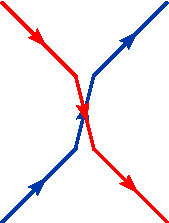
\includegraphics[width=3.0cm]{parton-showers/coherence7.pdf}}
    \hfill\raisebox{2cm}{(c)}\!\!
    \raisebox{30pt}{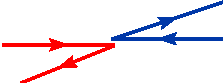
\includegraphics[width=4cm]{parton-showers/coherence8.pdf}}}
  \caption{As \FigRef{fig:hardscattercoherence} but for a quark
    scattering process.}
  \label{fig:hardscattercoherence2}
\end{figure}
The outgoing quark--antiquark pair has a distribution over all polar
angles, but the colour coherence effect is best illustrated by an event
in which the outgoing quark's direction is only a small angle away from
the incoming quark's (see \FigRef[c]{fig:hardscattercoherence}).  Although
the quark lines are annihilated and created, the colour lines are
scattered through small angles.  Detailed analysis supports the
intuition that one might derive from analogy with the Chudakov effect in
QED, that the radiation pattern from such an event is effectively that
of two independent colour lines, each of which is scattered through only
a small angle.  Such a small-angle scattering does not radiate at large
angles, only into a forward cone of opening angle given by the
scattering angle.  This event would not, therefore, radiate significantly at
central rapidities.

This radiation pattern should be contrasted with the one from a quark
scattering event with identical kinematics (\ie $qq'\to qq'$ at a small
angle, \FigRef{fig:hardscattercoherence2}).  In this process the
scattering takes place via a $t$-channel
gluon so that the colour of the incoming $q$ quark is carried through
the gluon on to the outgoing $q'$ quark and vice versa.  Therefore,
although the quarks have been scattered through a small angle, their
colour charges have been scattered through a large angle, almost
$180^\circ$, and they radiate throughout almost the entire event.  This
is actually the norm for small angle scattering, since it is dominated
by $t$-channel gluon exchange, but in the general case it is essential
that the colour connection of each parton is identified so that the
coherence of the different emitters can be incorporated.

The algorithm to set the starting scale of the shower from each parton
that implements this coherence
can therefore be stated as follows: trace the colour line of the parton
through the hard process to find the parton to which it is
colour-connected, the ``colour partner''.  Start the shower from each
parton with a maximum allowed opening angle given by the angle to the
colour partner.

A detailed analysis of three-jet events by the CDF
collaboration~\cite{Abe:1994nj}, showed that this colour coherence
effect is absolutely crucial to fit the data. They studied events with
three jets, the hardest of which had transverse energy\footnote{The transverse
  energy of a particle or jet is defined as $E_T=E\sin\theta$, where
  $E$ is its energy and $\theta$ is the polar angle of its direction of
  motion with respect to the beam axis.} $E_T>110$~GeV and the softest had
$E_T>10$~GeV, so that the sample was dominated by configurations with a
pair of roughly balancing high transverse energy jets and a relatively
soft third jet.  Distributions in the direction of this third jet were shown
to be particularly sensitive to the colour coherence effects in the
initial conditions of the shower.  Despite the fact that this analysis
was not corrected for detector effects, it is so important as a testing
ground for event generators that it has been implemented into \rivet
(see \SecRef{sec:rivet}) with
approximate detector corrections applied to the Monte Carlo events.  As an
example, we show in \FigRef{fig:CDFcoherence} the distribution of
$\eta_3$, the pseudorapidity of the third hardest jet.
\begin{figure}[tbp]
  \centering
  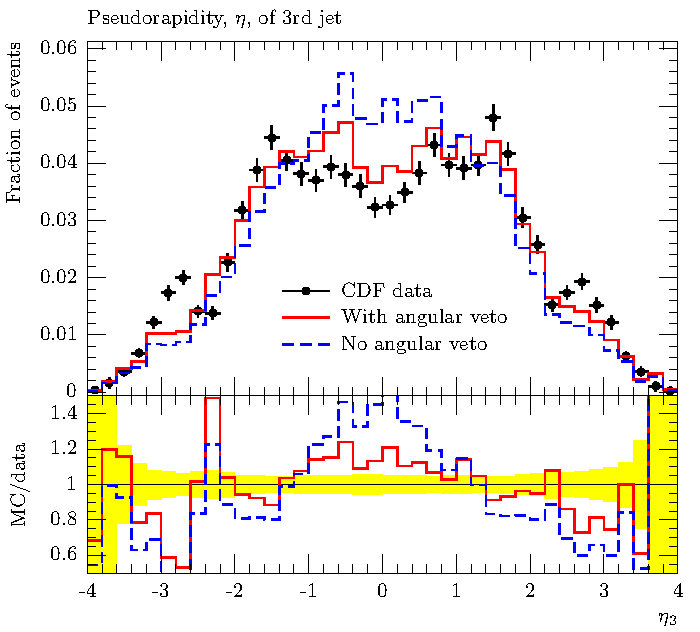
\includegraphics[scale=0.7]{mc-plots/CDF_1994_S2952106-inline/CDF_1994_S2952106_d03-x01-y01}
  \caption{CDF's evidence for colour coherence in $p\bar{p}$ collisions at
    $\sqrt{s} = 1.8$~TeV. The pseudorapidity of the 3rd jet is plotted,
    uncorrected for detector effects, with the \pythiasix Monte Carlo generator
    for comparison with angular vetoing turned on and off in the parton
    showers.}
  \label{fig:CDFcoherence}
\end{figure}
Since colour coherence is so inherent to modern generators, to illustrate this
effect we have had to return to \pythiasix with its old virtuality-ordered
parton shower (\pythiasix now preferentially uses a dipole shower ordered in
transverse momentum and \pythiaeight only includes this version, see
\SecRef{sec:pythia8}).  Results are shown with angular ordering of the first
initial-state emission switched off and on.  We see
that the dip in the data at central $\eta_3$ is not reproduced by
the Monte Carlo simulation unless angular emission ordering is imposed to account for
coherence effects.  The comparison of these data with the latest versions of the
main generators discussed in this review are shown in
\SecRef{sec:physics-areas-where}.

The general case of arbitrary $2\to2$ scattering is slightly more
complicated, because a given hard process may have more than one colour
flow.  For example quark--gluon scattering $qg\to qg$, has three Feynman
diagrams, with an $s$-channel or $u$-channel quark, or a $t$-channel
gluon.  One can show that there are two independent colour flows and,
for example, the colour flow of the $t$-channel diagram can be written
as the difference between the other two.  The amplitude associated with
each diagram is gauge-dependent, but the contribution of the sum of all
diagrams to the amplitude for a given colour flow is gauge-invariant and
is therefore physically meaningful.  Finally, one finds that the
interference between the amplitudes for different colour flows is always
suppressed by factors of the number of colours, $\Nc$, and therefore
that in the large-$\Nc$ limit (see \SecRef{sec:large-nc-limit}),
different colour flows can be considered
as independent physical processes.  One can therefore construct, for a
given hard process configuration, probabilities for it to be in each of
the colour flow states in the large-$\Nc$ limit.  Having chosen a given
colour flow, one can trace the colour lines through the hard process to
find the colour partner of each parton.  As shown in
\cite{Ellis:1986bv}, this procedure results in an emission
distribution that is correct up to terms that are suppressed not only by
at least $1/\Nc^2$, but are also dynamically suppressed, having no
collinear enhancement.

In the large-$\Nc$ limit, a gluon has two colour connections and in the
parton shower emits with colour factor $C_A$.  In the dipole approach of
\SecRef{sec:dipoles}, each line emits with a colour factor $C_A/2$, but
typically in coherent parton showers a different approach has been used:
One chooses one of the two colour partners with equal probabilities and
generates a parton shower with colour factor $C_A$ limited by the
opening angle to the chosen partner.  This procedure gives the correct
inclusive distribution of emission, but as shown in \cite{Schofield}
it produces too much event-to-event fluctuation,
the wrong rate for any number of exclusive emissions and, in particular,
a too high rate of non-emission.  The correct procedure is the more
dipole-like one in which each colour line emits with factor $C_A/2$ into
a cone limited by its colour partner.

We
make a final comment concerning the Lorentz invariance of the whole
procedure.  The coherence-improved parton shower described above was
formulated in terms of an evolution in opening angle, which is
manifestly not Lorentz invariant, but in practice it is usually
implemented as an evolution in the energy of the emitter times the
opening angle, $\tilde{q}\sim E\theta$.  In the soft and collinear
limits in which it is valid, this evolution \emph{is\/} Lorentz
invariant.  However, its starting condition is not.  In fact, one can
show, \cite{Ellis:1986bv}, that the initial conditions of two
colour-connected partons $i$ and $j$ are given by
\begin{equation}
  \label{eq:psinitialconditions}
  \tilde{q}_{i,\max}\,\tilde{q}_{j,\max} = p_i\cdot p_j.
\end{equation}
That is, depending on the choice of Lorentz frame in which the parton
showering is performed, the maximum value of evolution variable for
parton $i$, $\tilde{q}_{i,\max}$, and for parton $j$,
$\tilde{q}_{j,\max}$, may take any values, but they must be related by
\EqRef{eq:psinitialconditions}.  Although each shower is separately
frame-dependent, provided
colour-connected pairs of partons are developed in the same frame, the
shower of the whole event is Lorentz-invariant.  The same considerations
apply also to the separation between initial- and final-state showers.
One can think of the corresponding boosts as being like a gauge
transformation: changing the gauge moves radiation between different
legs but the sum of emission from all legs is gauge invariant.  This
reflects the fact we have mentioned several times that we use the
language of a classical branching process, because it is convenient, but
it is derived from the underlying quantum structure of the gauge theory.

\mcsubsection{Quark mass effects}
The parton showers we have described so far are for massless partons.
In this section we shall consider how they are modified by parton mass
effects.  Although we discuss the explicit case of quarks, our comments
are equally applicable to any massive coloured particle, for example
squarks and gluinos in supersymmetry.  We shall mainly consider the case
of scattering or production processes with momentum transfers
significantly larger than the quark mass since, as we shall see,
radiation is suppressed in the threshold region, where the invariant
mass of the coherent system of which the quark is a part is not much
larger than its mass.  We therefore work in a
Lorentz frame in which the quark's energy is large relative to its mass,
\ie its velocity is close to~$c$.  We defer a more technical
discussion of precisely how the quark mass is defined, which is
ambiguous beyond the leading order of perturbation theory, until
\AppRef{sec:top-quark-masses}.

In the soft limit, the universality of the amplitude to emit a gluon is
unaffected by the parton mass.  One can therefore derive a general
formula for the angular distribution of soft gluons emitted by a dipole
consisting of one or two massive (anti)quarks.  It has the property that
at large angles it is identical to the distribution produced by a
massless quark of the same total momentum.  This again accords with our
picture of colour coherence~-- a soft wide angle gluon is not able to
resolve the details of the colour line that emits it, all it sees is a
colour charge moving in a given direction.  The details of whether that
colour charge is carried by one parton or a bundle of collinear partons
and whether those partons are massless or massive do not affect it.  On
the other hand, the distribution is modified at small angles.  Defining
the ratio $m/E\equiv\theta_0$, which we assume to be small, we end up
with a distribution that is identical to that from a massless quark, but
with the replacement
\begin{equation}
  \label{eq:deadcone}
  \frac{\done\theta^2}{\theta^2} \rightarrow
  \frac{\theta^2\,\done\theta^2}{(\theta^2+\theta_0^2)^2}.
\end{equation}
We see that emission at large angles, $\theta\gg\theta_0$ is indeed
unaffected, but that it is suppressed at small angles, falling to zero
in the exactly forward direction.  In older parton shower algorithms,
such as \Herwig\ \cite{Marchesini:1989yk}, this was used as the basis for the
`dead cone approximation', in which the showering of massive partons was
performed in an identical way to massless ones, but with a cutoff on
opening angle at~$\theta_0$.  With an appropriate choice of frame in
which this evolution is performed, it can be shown to produce
approximately the right amount of radiation, but it is clearly too
brutal an approximation, producing too much radiation at angles a little
above $\theta_0$ and none at all below it.

While \EqRef{eq:deadcone} is derived in the high energy limit,
$\theta_0\ll1$, it shows that near threshold, where $\theta_0\sim1$,
emission is suppressed at all angles.  Indeed, the more general
expression from which it is derived shows that at large angles, the
emission probability is proportional to the velocity-squared of the
emitting partons and hence that it goes to zero at threshold.

Ref.~\cite{Norrbin:2000uu} considered the matrix elements for gluon
emission in the decay of heavy objects to lighter partons with various
colour, spin and parity quantum number assignments.  It was found that the
radiation pattern for finite gluon energy, while always suppressed in
the forward direction, is significantly dependent on all of these
parameters and in most cases not going exactly to zero even in the
collinear limit.  These are implemented in \Pythia as process-dependent
mass corrections.

The authors of Ref.~\cite{Catani:2002hc} derived a generalization of the DGLAP splitting
function to the massive case, which they called the quasi-collinear
limit.  This is defined as the limit of $p_t^2\sim m^2\ll Q^2$, where
$Q^2$ is the hard scale.  They found
\begin{equation}
  \hspace*{-1cm}
  \begin{array}{rcl@{\hspace*{2.5em}}rcl}
    P_{QQ}(z) &=& C_F\left[\frac{1+z^2}{1-z\phantom{^2}}-\frac{m^2}{p_Q\cdot p_g}\right], &
    P_{gQ}(z) &=& T_R\left[z^2+(1-z)^2+\frac{2m^2}{(p_Q+p_{\bar{Q}})^2}\right].
  \end{array}
  \hspace*{-1cm}
\end{equation}
These are such that the subsequent limit $m\to0$ at fixed \pt\ smoothly
recovers the massless behaviour.  The limit $\pt\to0$ at fixed $m$
corresponds to the soft limit, if at fixed opening angle, and reproduces
\EqRef{eq:deadcone} or the collinear limit, if at fixed energy, and
recovers the result of Ref.~\cite{Norrbin:2000uu} for the generalization of
the dead-cone suppression to finite energy.  The quasi-collinear
splitting functions are used in \Herwigpp and \Sherpa, while the
matrix-element correction method of \cite{Norrbin:2000uu} is used in
\pythiaeight.

\mcsubsection{The dipole approach to parton showering}
\label{sec:dipoles}
In discussing the parton shower approach to simulating radiation from
the partons involved in a scattering process, we mentioned several times
the alternative formulation in terms of emission from sets of colour
dipoles.  This approach was first used in the \Ariadne\ program
\cite{Gustafson:1987rq}, described in more detail in
\SecRef{sec:ariadne}, and in fact is used by the majority of recent new
implementations, including \pythiaeight \cite{Sjostrand:2004ef}, see
\SecRef{sec:pythia8}, and \sherpa, with a choice of two different dipole
shower implementations, \cite{Winter:2007ye,Schumann:2007mg}, see
\SecRef{sec:sherpa}, as well as several standalone dipole cascade programs
\cite{Giele:2007di,Nagy:2007ty,Dinsdale:2007mf}.  For most
purposes it can be considered equivalent to the coherence-improved
parton showers discussed already, but it does have some advantages,
which we briefly describe in this section.

The basic observation is that, as discussed in
\SecRef{parton-shower:initial-conditions} and in more detail in
\SecRef{sec:cluster-model}, in the large-$\Nc$ limit the
colour structure of an arbitrarily-complicated system of partons can be
decomposed as a colour flow, \ie a set of colour lines each starting on an
incoming quark, outgoing antiquark or gluon, connecting it with an
outgoing quark, incoming antiquark or other gluon, and that in the
soft-gluon and large-$\Nc$ limits, each of these lines emits
independently.  Whether the configuration was produced by a
matrix-element calculation or by the parton shower itself, one can
calculate, again in the large-$\Nc$ limit, the probabilities of
different colour flows and hence choose in a given event a particular
colour flow.  One can quantify the validity of the dipole approximation
as being the limit in which the transverse momentum of the emitted
gluon, relative to the axes defined by the colour line from which it is
emitted, is much smaller than any scales involved in the production of
that colour line.  It is therefore natural to use transverse momentum as
the ordering variable for dipole showers.

The procedure is then to start from the hard process, decompose its
colour structure as described in
\SecRef{parton-shower:initial-conditions} and choose one colour flow.
This gives a unique initial condition for the subsequent dipole
evolution.  Each colour line connecting a pair of partons effectively
forms a colour--anticolour dipole and the emission from each dipole is
generated independently.  Although in the soft limit each dipole emits
independently with a classical radiation pattern, emission with a finite
transverse momentum results in a recoil.  Since a gluon carries the
colour lines of two dipoles, any recoil it experiences may affect the
subsequent evolution of the neighbouring dipoles.  Therefore the event
is evolved globally, with the highest transverse momentum emission from
any dipole being generated first, complete with its recoil, and its
transverse momentum giving the upper limit for the subsequent evolution
of the ensemble of dipoles.  Although this shower is formulated in the
soft limit, it was shown by \cite{Gustafson:1987rq} that
collinear effects can be incorporated in the large-$\Nc$ limit by a
simple modification to the rapidity distribution of the emitted gluon
(which is flat in the soft limit).  Recent implementations have gone
further by using the dipole splitting functions and kinematics defined
in the dipole subtraction method \cite{Catani:1996vz} to partition each dipole
into `monopole' pieces related to each of the two emitters of the dipole
(with the other taking the role of spectator) each with its own colour
factor, so that the collinear limit is exact in $\Nc$ and, like the
coherence-improved parton shower, neglected terms are both $\Nc^2$ and
dynamically suppressed.

Some doubt was cast on the validity of the dipole shower method in
Ref.~\cite{Dokshitzer:2008ia}, but it may be that the problem found
there is an artefact of the toy model
used \cite{Nagy:2009re,Skands:2009tb} and is not shared by full
implementations.  To our
understanding, transverse-momentum-ordered dipole showers with collinear
improvement are accurate to leading-collinear-logarithmic order and
hence are formally as accurate as angular-ordered parton showers.

In fact, despite this formal equivalence, the dipole shower has some
practical advantages.  Firstly, the fact that it is transverse momentum
ordered means that the hardest emission is generated first, making
matrix element corrections significantly more straightforward to
implement and obviating the need for truncated showers (see
\SecRef{sec:me-nlo-matching}) from the internal lines.  Secondly, the
fact that emission is a $2\to3$ process, rather than $1\to2$, means that
energy-momentum can be explicitly conserved, with all external partons
on mass shell, at each step of the shower.  In the parton shower approach,
the initially on-shell parton develops some virtuality and momentum
conservation must be violated at intermediate steps of generation.  Only
once all partons have developed their showers is a small amount of
momentum shuffled between partons to restore its conservation.  Finally,
the problem mentioned in \SecRef{parton-shower:initial-conditions}, of
how to generate emission from the two colour lines of a gluon is
obviated, since they simply radiate independently in the dipole
approach.
The kinematic variables used in dipole showers are Lorentz invariant and
they naturally combine the radiation from colour-connected parton pairs,
hence the issues discussed at the end
of \SecRef{parton-shower:initial-conditions} are automatically satisfied
by dipole showers.

We finally mention the extension of the dipole method to initial-state
radiation.  In the original implementation
in \Ariadne~\cite{Lonnblad:1992tz}, \SecRef{sec:ariadne}, there was no
explicit initial-state radiation.  The outgoing hadron remnant acted as
an emitter at one end of a dipole like any other parton except that,
being an extended object, radiation in its collinear direction was
suppressed.
%% This approximately mimicked the effect in the backward
%% evolution algorithm of valence quark distributions, which suppress
%% radiation from high-$x$ partons, but there is no explicit mechanism to
%% match the distribution with an input DGLAP-evolved PDF set.  Following
%% emission from a remnant dipole, the remnant itself does not take any
%% recoil, but rather, it emits a low-momentum gluon that takes its recoil,
%% which was shown to mimic some of the features of CCFM
%% evolution~\cite{Lonnblad:1992tz}.
More recent dipole showers have formulated the evolution of dipoles
containing an initial-state emitter in a more backward-evolution-like
way, guided by the PDF set.
%% However, a potential feature of this approach is the
%% fact that, in the evolution of Drell--Yan events for example, the
%% description of low transverse momentum events can be at odds with the known
%% asymptotic behaviour of the QCD cross section~\cite{Parisi:1979se}.  The
%% starting configuration is an initial--initial dipole, so that the
%% produced $\gamma^*/W/Z$ boson absorbs the recoil from the hardest
%% emission.  This emission splits the dipole into two initial--final
%% dipoles and the simplest implementation of the subsequent evolution
%% shares the recoil between the
%% partons without affecting the boson's momentum.
%% This is in contrast to the QCD behaviour, in which the full
%% Feynman-diagrammatic approach shows that resummation of multiple
%% emissions is essential to describe the low-$p_t$ region and the Sudakov
%% exponentiation implied by including only the hardest gluon is not
%% sufficient.  As discussed in
%% Ref.~\cite{Nagy:2009vg}, it is possible in principle to define
%% dipole-like algorithms that solve this problem by allowing the whole
%% event to absorb the recoil from each emission and \pythia and \sherpa
%% have both implemented solutions to this problem.

\mcsubsection{Summary}

\begin{itemize}
\item Scattered, annihilated and created partons radiate gluons.
\item Since gluons themselves are coloured, this radiation gives rise to
  further gluon radiation and parton multiplication.
\item These showers can be simulated as an evolution in some
  appropriately chosen scale down from the scale of the hard process
  towards an infrared scale at which non-perturbative confinement
  effects set in.
\item This evolution effectively sums to all orders terms enhanced by
  logarithms of the hard and soft scales, and can be formulated as
  coherence-im\-proved parton showers or transverse-momentum-ordered
  dipole showers.
\item Modern algorithms are extremely sophisticated implementations of
  all-order perturbative QCD.  Although they use the probabilistic
  language of time-ordered sequential emission, they are derived from
  the full quantum structure of the underlying gauge theory, QCD.
%Describing emission as
%being from a given parton or dipole is convenient, but is not physically
%meaningful, only the sum of emission from all emitters in the event is.
\end{itemize}

Nevertheless, parton shower algorithms are certainly not the whole story
in describing the exclusive structure of an event.  Firstly, they are
built on soft and collinear approximations to the full cross sections,
while many of the observables we are interested in are explicitly
sensitive to hard wide-angle emission and multi-jet final states, which
can only be described accurately with the help of higher-order matrix
elements, as discussed in \SecRef{sec:me-nlo-matching}.  And secondly,
they cannot be extended arbitrarily far into the infrared region where
QCD becomes strongly-interacting and must be cut off at some scale
beyond which non-perturbative models for hadronization and the
distributions of partons in incoming hadrons (\ie PDFs and primordial
$k_\perp$) must be invoked, as described in
\SecsRef{sec:minim-bias-underly} and \ref{sec:hadronization}.

% Local Variables:
% mode: LaTeX
% TeX-master: "../mcreview"
% End:
